\chapter{Soluzione proposta}
% \chapter{16}
 %\label{chapter:our_work}

\section{Introduzione}
%spiegare obiettivo
Il nostro obiettivo è di creare un sistema di anomaly detection con struttura distribuita: nei router delle sedi periferiche dell'azienda vengono raccolte informazioni sul traffico e in un server posizionato fisicamente nella sede centrale vengono analizzati e in base al risultato vengono prese decisioni sulle future azioni da intraprendere. Questa tipologia di architettura permette di sfruttare dispositivi già esistenti e non aggiunge molta complessità all'infrastruttura informatica aziendale, quindi per svolgere questo lavoro ci siamo basati su alcuni software e sull'hardware aziendale con i relativi vantaggi e svantaggi rispetto ad una soluzione completamente ex-novo.
Inoltre essendo una soluzione distribuita permette di bloccare gli attacchi e il traffico malevolo lontano dalla sede centrale, in modo da essere più efficace e non influenzare il comportamento di altre sedi in caso di un attacco proveniente da una o più sedi periferiche.
% spiegare come vengono gestiti i dati
La raccolta e l'analisi dei dati viene effettuata utilizzando un sistema centralizzato, questo permette di avere un unico dispositivo con la capacità necessaria a svolgere l'elaborazione, che al tempo stesso possiede una visione completa sulle sorgenti e quindi sarà in grado di identificare facilmente da quale sede proviene il traffico anomalo.


\section{Gestione dei dati}

I dati vengono collezionati tramite un demone sui router (collectd), inviati ad un server (go-graphite) e visualizzati tramite una dashboard (Grafana). Il tool di anomaly detection da noi sviluppato si interfaccia direttamente con il database per la lettura dei dati e la scrittura dei risultati.
Qui in seguito approfondirò maggiormente il flusso della gestione dei dati.

\begin{figure}[]
    % todo: capire come gestire citazioni imsmagini a livello di copyright
    %  e capire come funzionano le label per richiamare le immagini
    \label{fig:mos}
    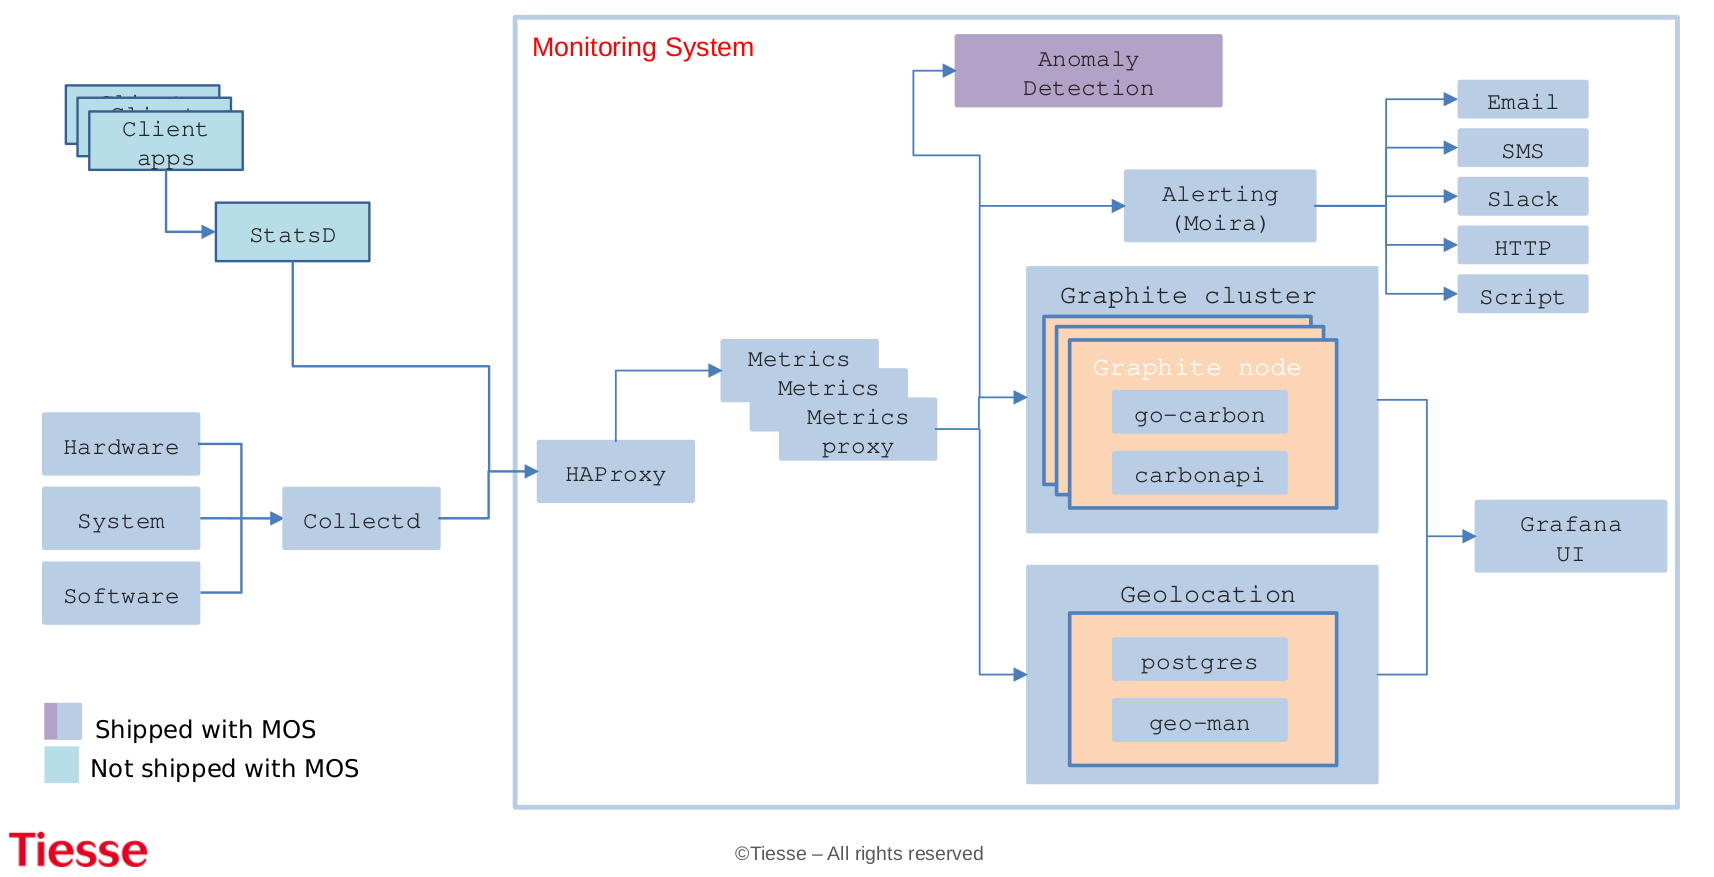
\includegraphics[width=\hsize]{images/my_work/tiesse_mos.png}
    \caption{Architettura di MOS (Monitor System di Tiesse)}
    \centering
\end{figure}

\subsection{collectd}

\begin{figure}[]
    % todo: capire come gestire citazioni imsmagini a livello di copyright
    %  e capire come funzionano le label per richiamare le immagini
    \label{fig:collectd}
    \begin{center}
        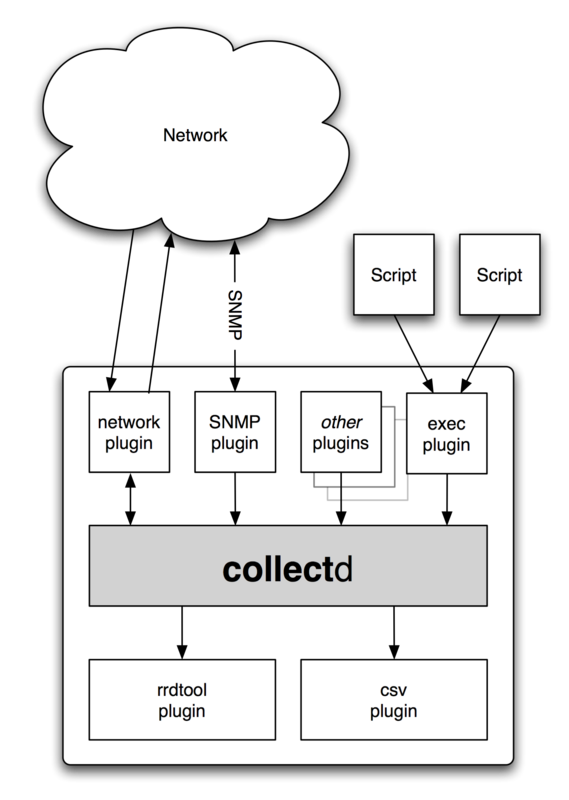
\includegraphics[height=300pt]{images/my_work/collectd.png}
    \end{center}
    \caption{Architettura di collectd}
    \centering
\end{figure}

Collectd è un demone che raccoglie metriche di sistema e di applicazioni, trasferisce e salva dati di computer e dispositivi di rete. Collect ha una struttura modulare, vedi figurra \ref{fig:collectd} in cui è possibile abilitare centinaia di plugin per la raccolta di metriche di sistema dai casi più generali a quelli più specifici ed inoltre è possibile scrivere i propri plugin per integrarlo ulteriormente. I plugin usati sono ``write\_graphite'': plugin che permette di scrivere le metriche raccolte su un database graphite, ``conntrack'': plugin che permette di contare il numero di voci nella connection tracking table di Linux, ``interface'' : plugin che colleziona informazioni sul traffico su un'interfaccia, quindi pacchetti al secondo, bytes al secondo ed errori sull'interfaccia. 

Inoltre per avere ulteriori dati a disposizione ho scritto un plugin che si occupa di aggiungere delle metriche sul conteggio dei pacchetti non possibile con i plugin standard.




\subsection{NDPI} 
NDPI è un software open-source per il deep-packet inspection basato su OpenDPI, il suo scopo è di riconoscere protocolli conosciuti anche su porte non standard, \uline{inoltre può essere personalizzato per il riconoscimento di applicazioni aziendali (è vera questa cosa?)}. nDPI è implementato nei router Tiesse e permette l'analisi dei pacchetti senza un degrado prestazionale.
%http://luca.ntop.org/nDPI.pdf
%todo: completare ndpi


\subsection{graphite} è un software open source per il monitoraggio che può funzionare sia su hardware economico, che su un'infrastruttura cloud. Può essere usato per monitorare le performance di siti, applicazioni, server e nel caso di Tiesse è usato per monitorare informazioni sull'uso dei router, come per esempio il numero totale di router connessi, quelli raggiungibili, il throughput, l'uptime e la velocità della connessione xDSL.
L'obiettivo di graphite è il salvataggio di serie temporali di dati numerici e la successiva condivisione e visualizzazione.
Graphite è composto da tre parti (come si può vedere dalla figura ~\ref{fig:graphite}):

% https://www.aosabook.org/en/graphite.html
% https://graphiteapp.org/#gettingStarted
%todo: spiegare meglio come funzionano le carbon api
\begin{itemize}
    \item carbon: è un service ad altre prestazioni che si occupa di ricevere le metriche con formato ``(timestamp, value)'' da salvare.
    \item whisper: un semplice database che salva sul filesystem le sequenze temporali di dati.
    \item graphite-web: è un'interfaccia utente e delle API le quali restituiscono i dati per renderizzare i grafici da visualizzare.
\end{itemize}

\begin{figure}[h]
     \label{fig:graphite}
    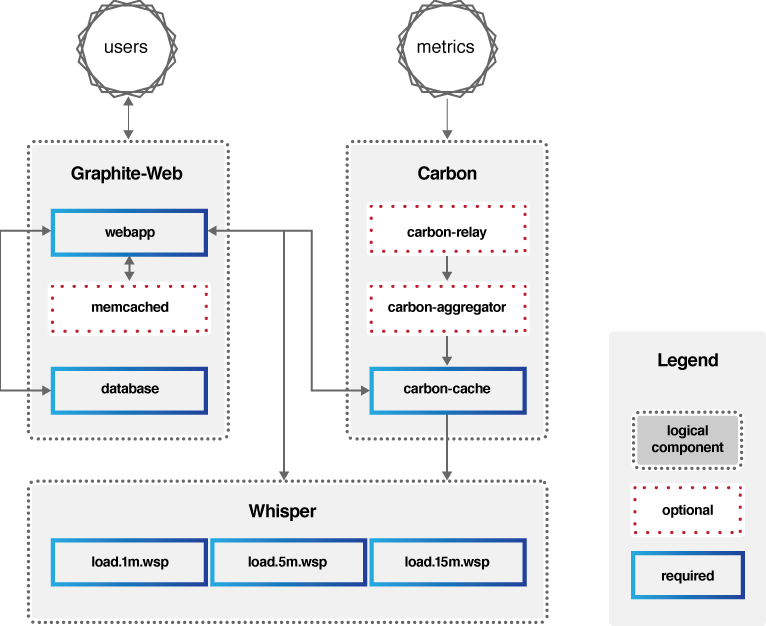
\includegraphics[width=\hsize]{images/my_work/graphite.png}
    \caption{Architettura di Graphite}
    \centering
\end{figure}

\paragraph{go-graphite} è un'implementazione in Golang di Graphite, rispetto alla versione originale di carbon il backend
go-carbon è più veloce in tutte le condizioni (la differenza di prestazioni varia in base alla macchina su cui è installato) ~\ref{fig:gocarbon}.
Le carbonapi invece sono un subset delle api di graphite-web e le vanno a sostituire essendo dalle 5 alle 10 volte più veloci.

\begin{figure}[h]
    % todo: capire come gestire citazioni imsmagini a livello di copyright
    %  e capire come funzionano le label per richiamare le immagini
    \label{fig:gocarbon}
    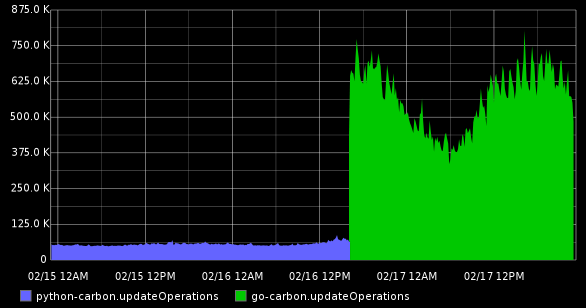
\includegraphics[width=\hsize]{images/my_work/go-carbon.png}
    \caption{Differenza di prestazioni tra carbon e go-carbon}
    \centering
\end{figure}
% https://github.com/go-graphite/go-carbon


\begin{figure}[h]
    % todo: capire come gestire citazioni imsmagini a livello di copyright
    %  e capire come funzionano le label per richiamare le immagini
    \label{fig:grafana}
    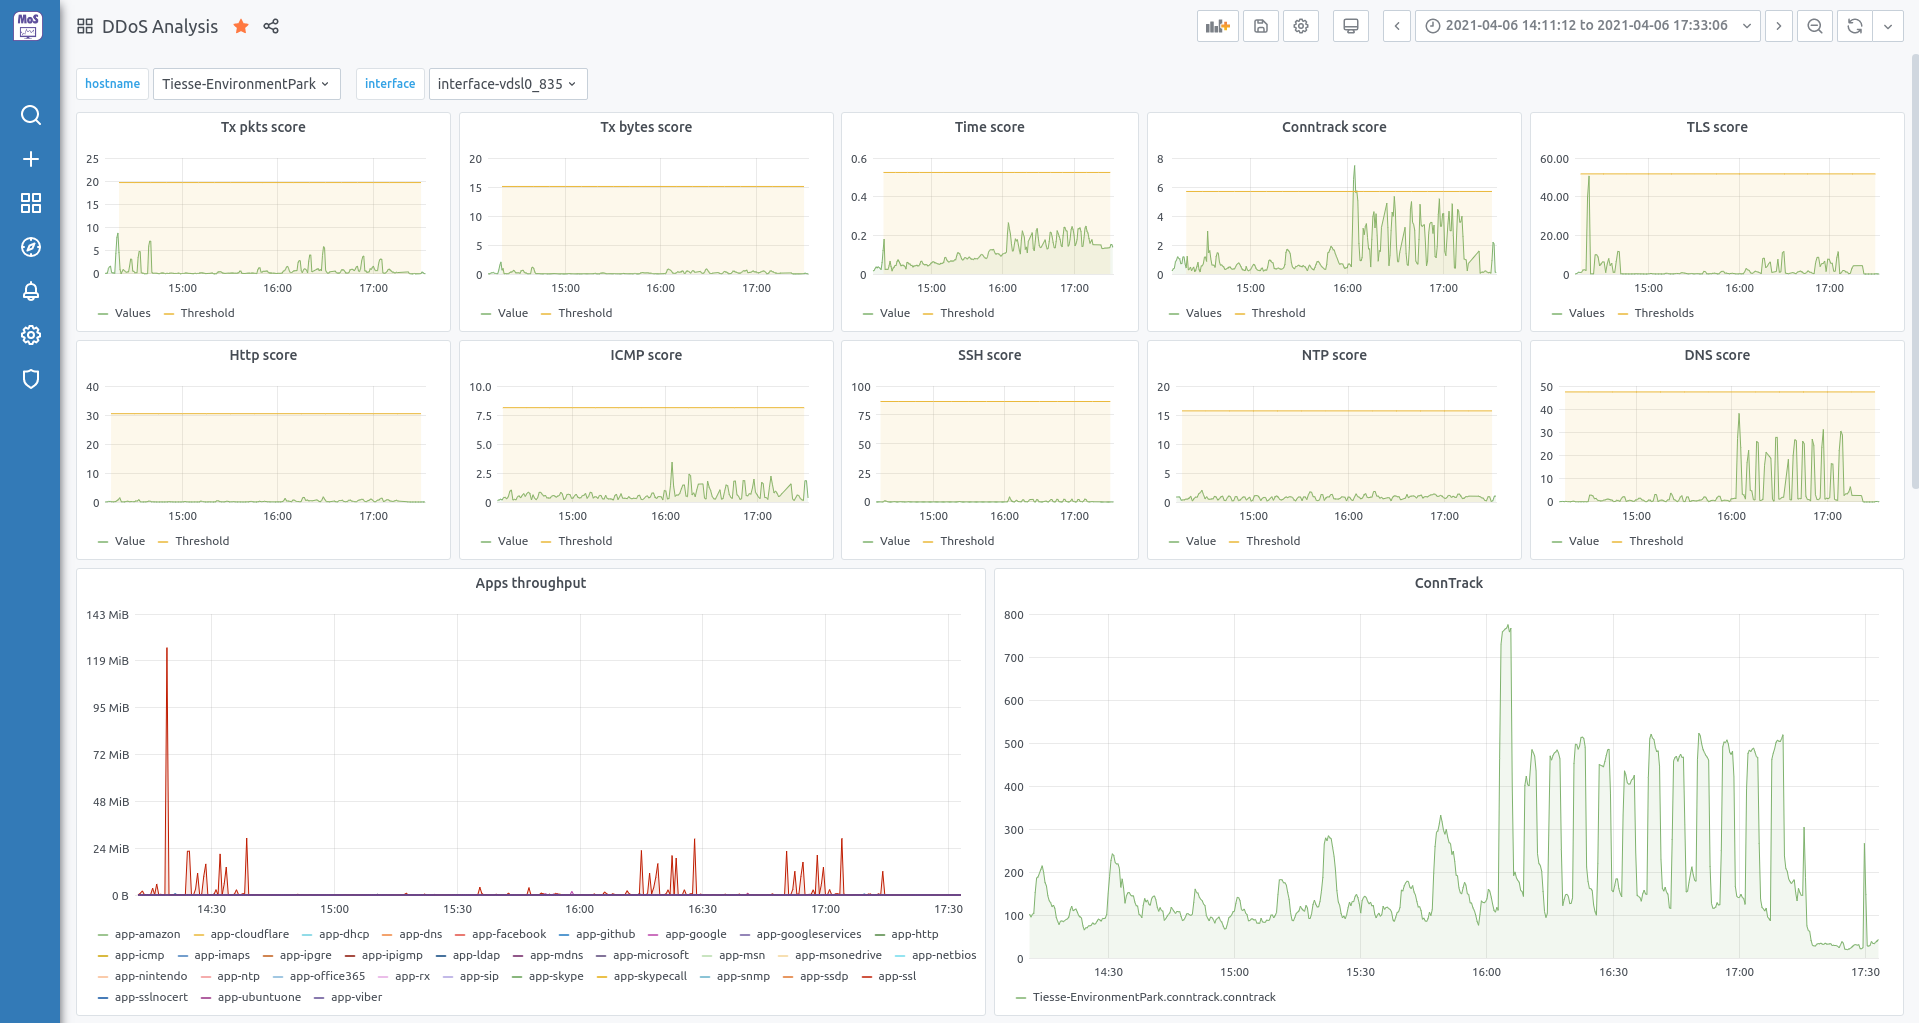
\includegraphics[width=\hsize]{images/my_work/grafana_dashboard.png}
    \caption{La dashboard per l'anomaly detection su Grafana}
    \centering
\end{figure}

\subsection{Grafana} è un software open source che permette la visualizzazione e la generazione delle metriche tramite una web application. Permette di creare dashboard dinamiche interrogando le api di graphite-web. Nel mio caso ho organizzato una dashboard in modo da visualizzare sia i dati provenienti dai router da analizzate, sia gli anomaly score calcolati dal software di anomaly-detection ~\ref{fig:grafana}.


%todo: come vengono mandati i dati di ndpi?
Riassumendo i dati provenienti dai plugin di collect, dal mio plugin e da NDPI vengono collezionati da collectd e inviati tramite il plugin write\_graphite al backend go-carbon, che si occupa di ricevere i dati e salvarli sul file system. Per la visualizzazione dei dati viene usato grafana, che permette di visualizzare i dati richiedendo i dati alle carbonapi e contemporaneamente il mio tool di anomaly detection richiede i dati per analizzarli, ogni volta che ottiene dei risultati li manda a go-carbon per salvarli nel database ~\ref{fig:mos}.
% todo: approfondire MOS
% todo: fare immagine con la gestione dei dati


\section{Selezione features}

La scelta delle feature da utilizzare dipende da quale obiettivo su vuole ottenere, il mio obiettivo primario in questa tesi è di rilevare gli attacchi DDoS in uscita verso la sede centrale, quindi basandomi sugli attacchi più famosi e frequenti ho delineato una lista di parametri da osservare. Questi parametri sono:
% todo: capire le unità di misura i dati sono ogni secondo o ogni 10
\begin{itemize}
    \item \emph{bytes trasmessi al secondo}:questa metrica è utile, abbinata ad altre, per la rilevazione di attacchi che mirano alla saturazione della banda.
    \item \emph{pacchetti trasmessi al secondo}: questa metrica ha uno scopo simile alla precedente oppure aiuta ad avere informazioni sugli attacchi di tipo flooding.
    \item \emph{numero di connessioni aperte}: il numero di connessioni aperte è un indicatore importante per identificare tutti gli attacchi che mirano a saturare le connessioni di un server. %todo: questa ha molti usi
    \item \emph{numero di pacchetti con flag syn}: questa metrica è molto utile per la rilevazione di syn flood o port scanning.
    \item \emph{tls throughput}: tutto il traffico inviato su un canale sicuro tls non può essere analizzato più nello specifico, quindi viene raggruppato in questa categoria.
    \item \emph{dns throughput}: conoscere il traffico relativo al traffico dns può essere utile come indice di un attacco contro il server DNS aziendale oppure di un attacco di DNS amplification.
    \item \emph{ssh throughput}: potrebbe segnalare anomalie sull'utilizzo improprio di macchine nella sede centrale tramite delle connessioni ssh.
    \item \emph{ntp throughput}: potrebbe segnalare anomalie riguardanti attacchi DDoS di NTP amplification.
    %todo: da rivedere come funzionano gli icmp durante un syn flood
    \item \emph{icmp throughput}: è un indicatore di attacchi, per esempio durante un syn flood usando ip spoofing, con ip della sottorete dell'attaccante, al ritorno dei syn ack si vede un aumento degli icmp che indicano che l'host non è esistente o che la porta destinazione a cui è destinato il pacchetto è chiusa. Inoltre gli icmp possono anche essere usati direttamente per degli attacchi.
    \item \emph{ora del giorno}: l'ora del giorno viene aggiunta per caratterizzare al meglio il traffico lungo la giornata.
    %todo: aggiungere http e ntp
\end{itemize}

Tutte le feature vengono poi \uline{derivate su un tempo di 10/30s, per avere dei "rate"} confrontabili tra lavoro.

La scelta della features è nata da un compromesso tra i dati necessari per rilevare al meglio le anomalie, la riduzione dei dati da salvare sul server e di conseguenza l'uso di banda usata per il trasferimento. Inoltre un problema che ho dovuto tenere in considerazione è l'utilizzo di un \underline{acceleratore hardware} nei router Tiesse, il quale permette un incremento della velocità di routing, ma non permette di analizzare nel kernel i pacchetti.
 %todo: approfondire meglio come funziona il fast path
 
\section{Il nostro tool}

Per una migliore raccolta e monitoraggio di features con diversa granularità, abbiamo sviluppato un ulteriore software in grado di estrarre metriche relative a \uline{server/servizi} aziendali specifici o metriche non disponibili tramite i plugin ufficiali di collectd, come per esempio il syn rate. Per svilupparlo abbiamo programmato un modulo kernel, che comunicava con un plugin per collectd da noi creato tramite un process file system (procfs), per una discussione più approfondita rimando al capitolo 5.

Questa soluzione è funzionante ed è stata testata in laboratorio, però non viene utilizzata per la raccolta di dati necessaria a causa dell'impossibilità di introdurre software aggiuntivo in un router in produzione, da cui dipendeva la produttività dell'ufficio. Inoltre i router Tiesse sfruttano un acceleratore hardware, in cui solo il primo pacchetto di ogni flusso passa tramite il kernel e i successivi vengono inoltrati automaticamente in hardware.
% Cosa fa?
% Perchè l'ho fatto?

% todo: perchè è commentata?
% Per rilevare le anomalie, una volta decise le features da analizzare, abbiamo dovuto decidere quale sistema dei precedentemente elencati adottare. La scelta è ricaduta sull'utilizzo di una rete neurale di autoencoder, la quale permette di allenare facilmente il modello in modo semi-supervisionato, grazie all'utilizzo della sola classe normale di traffico.

\subsection{Struttura}

% Posso parlare di come è strutturato il programma, che librerie ho usato 
Il programma è scritto in Python 3, con l'utilizzo di TensorFlow e Keras librerie per il ``machine learning'', effettua le richieste http tramite la libreria requests e gestisce i dati grazie a NumPy e Pandas: librerie per il calcolo matriciale e la gestione di tabelle e serie.
Il tutto, per assicurare una maggiore portabilità, ed assicurare la possibilità di effettuare il deploy su qualsiasi macchina, viene eseguito all'interno di un container Docker, la cui immagine viene creata e avviata tramite ``docker-compose''.


I dati all'interno del repository sono organizzati nel seguente modo:

\dirtree{%
.1 /.
.2 data\DTcomment{Cartella dove verrà salvato il modello e le immagini generate}.
.2 src\DTcomment{Cartella con i sorgenti del programma}.
.3 requirements.txt\DTcomment{Librerie di python necessarie}.
.3 utility.py \DTcomment{File in cui sono presenti le funzioni comuni}.
.3 update\_db.py \DTcomment{Funzioni per caricare i risultati su graphite}.
.3 evaluate.py \DTcomment{File con le funzioni per valutare se sono presenti anomalie}.
.3 train.py \DTcomment{File con funzioni per eseguire l'allenamento della rete}.
.3 model.py \DTcomment{File con funzioni per generare il modello}.
.3 test.py \DTcomment{Script che esegue la creazione di un modello, il train e la successiva valutazione di anomalie, basandosi su un file di impostazioni}.
.3 main.py \DTcomment{Script che esegue la creazione e il train del modello se non presente e a intervalli regolari verifica le anomalie}.
.2 test\_configs.
.3 test\_docs\_v3.json\DTcomment{Un esempio di file di configurazione usato per effettuare i test della validità del modello}.
.2 Dockerfile.
.2 docker-compose.yml.
.2 README.md.
}
\subsection{Keras e TensorFlow}

\paragraph{Tensorflow 2} è una libreria open-source sviluppata da Google per il machine learning che fornisce moduli ottimizzati per la realizzazione di algoritmi di machine learning e la loro esecuzione in maniera efficiente su CPU, GPU e TPU. Inoltre permette di scalare agevolmente su un'architettura con molti device.
% \cite{keras_about}

\paragraph{Keras} è un insieme di API ad alto livello di TensorFlow 2 che forniscono astrazioni essenziali per incentrarsi sulla facilità d'uso, la modularità e l'estendibilità per la risoluzioni di problemi relativi al machine learning, con una particolare concentrazione sui moderni problemi di deep learning.


\subsection{Elaborazione dei dati in input}
% Come ricevo i dati dal server? Come li elaboro? Che api uso?
% Genero tante piccole sequenze di 8 elementi (spiegare il motivo della scelta della sequence length => trade-off tra tempo di rilevamento dell'anomalia e mitigazione dei picchi e dei falsi positivi) e perchè lo faccio, come normalizzo i dati e perchè. Come fornisco i dati in input alla rete.


Le metriche relative alle applicazioni vengono aggiornate ogni 30 secondi, a differenza dei 10 secondi con cui aggiorno i dati collezionati da collectd, per questo motivo ogni volta che devo richiedere dei dati al server devo effettuare due richieste, tramite la libreria requests, alle carbonapi.

% (Viene usato http con basic auth, questo mi provoca un colpo al cuore lato sicurezza, ma lo posso giustificare dicendo che è un ambiente di test, in produzione come minimo verrà usato https.)

Un esempio di dati restituiti dalla prima richiesta è mostrata nel codice \ref{code:carbonapijson}, in cui per ridurre la quantità di dati da mostare nell'esempio, ipotizzo che l'intervallo di tempo richiesto sia di venti secondi.

\begin{lstlisting}[language=json,caption={Esempio di risposta delle carbonapi}\label{code:carbonapijson}]
[
    {
        "target": "Tiesse-EnvironmentPark.conntrack.conntrack",
        "datapoints": [
            [
                135,
                1619681610
            ],
            [
                134,
                1619681620
            ]
        ],
        "tags": {
            "name": "Tiesse-EnvironmentPark.conntrack.conntrack"
        }
    },
    {
        "target": "Tiesse-EnvironmentPark.interface-vdsl0_835.if_packets.tx",
        "datapoints": [
            [
                21.199091,
                1619681610
            ],
            [
                26.401902,
                1619681620
            ]
        ],
        "tags": {
            "name": "Tiesse-EnvironmentPark.interface-vdsl0_835.if_packets.tx"
        }
    },
    {
        "target": "Tiesse-EnvironmentPark.interface-vdsl0_835.if_octets.tx",
        "datapoints": [
            [
                4202.222148,
                1619681610
            ],
            [
                5862.413248,
                1619681620
            ]
        ],
        "tags": {
            "name": "Tiesse-EnvironmentPark.interface-vdsl0_835.if_octets.tx"
        }
    }
]
\end{lstlisting}
I dati ricevuti per essere elaborati devono essere memorizzati in una tabella con il corretto formato, vedi l'esempio di tabella \ref{table:tabella_dati_1}, per questo motivo i dati del json appena ricevuto vengono elaborati, sostituendo per prima cosa il timestamp, il quale viene trasformandolo da un unix timestamp ad uno che indica i secondi passati dalla mezzanotte e successivamente tutti gli elementi verranno aggiunti ad un dizionario con il corretto formato, come mostrato nell'estratto di codice \ref{code:get_data}.

% todo: e i syn?
\begin{table}[]

\begin{tabular}{||c c c c c||} 
\hline
index & timestamp  & .conntrack.conntrack & ..if\_packets.tx & ..if\_octets.tx \\ [0.5ex] 
\hline\hline
1 & 45810 & 71.0 & 7.500424 & 2416.445886 \\ 
\hline
2 & 45820 & 74.0 & 4.89923 & 51069.831629415 \\
\hline
3 & 45830 & 72.0 & 5.000281 & 1224.055123 \\
\hline
\end{tabular}
\caption{Tabella di esempio dei dati ricevuti relativi alle features di collect.}
\label{table:tabella_dati_1}
\end{table}
% \begin{lstlisting}[language=csv]
% ,timestamp,.conntrack.conntrack,..if_packets.tx,..if_octets.tx
% 0,45810,181.0,38.902328,6055.20679
% 1,45810,181.0,38.902328,6055.20679
% \end{lstlisting}

% todo: come metto le lettere accentate?
\begin{lstlisting}[language=python3, label={code:get_data}, caption={Funzione usata per scaricare i dati dal server}]
def get_data(s_time, e_time, hostname: str, interface: str,
    username: str = None, password: str = None):
    r = requests.get(
    f"http://{host}:{port}/api/datasources/proxy/4/render?"
    f"target={'&target='.join(target_list(hostname,interface))}"
    f"&from={s_time}&until={e_time}&format=json",
    auth=HTTPBasicAuth(username, password)
    )
    # se il valore ritornato non e' 200 OK viene
    # lanciata un'eccezione, gestita a livelli superiori
    print(r.status_code, '-', r.url)
    if r.status_code != 200:
        raise Exception('Get features data error')

    # converto la risposta in un json 
    # e poi in un dizionario con chiave il target
    # e come valore i datapoints
    json_resp = r.json()

    # todo: probabilmente ci sono modi piu' efficienti
    data = data_to_dict(json_resp)
    data_list = list()
    for i in range(len(json_resp[0]['datapoints'])):
        line: dict = dict()
        timestamp =
        datetime.fromtimestamp(json_resp[0]['datapoints'][i][1])
        # trasformo il tempo in secondi dalla mezzanotte
        line['timestamp'] = timestamp.hour * 3600 \
                            + timestamp.minute * 60 \
                            + timestamp.second
        tl = target_list(hostname, interface)
        for e in tl:
            line[e] = data[e][i][0]
        data_list.append(line)

    # creo la matrice con pandas ed elimino le righe con valori
    # mancanti in rari casi le carbon api mi restituiscono dei
    # valori nulli, per questo motivo cancello le righe in cui
    # c'e' almeno un valore nullo
    matrix = pd.DataFrame(data_list).dropna()

    # successivamente richiedo anche i dati delle app, e quando
    # li ricevo, dopo averli manipolati, li unisco tutti
    # in un'unica tabella
    app_data_matrix =
    get_app_data(s_time, e_time, hostname, username, password)

    matrix = pd.merge(app_data_matrix, matrix)

    # questa funzione mi permette di ritornare l'elenco 
    # delle feature attualmente utilizzate, senza impostare
    # host e interfaccia da utilizzare
    matrix.columns = total_target_list('', '')
    return matrix

\end{lstlisting}

Ricevuti i dati e organizzati nel formato corretto, effettuo una nuova richiesta alle carbon api, per ricevere le statistiche relative alle applicazioni, il procedimento è simile a quello precedentemente descritto, l'unica differenza è che i dati sul database vengono salvati da ndpi ogni 30 secondi, per questo motivo devo estenderli mostrando lo stesso dato più volte, in modo da avere lo stesso numero degli elementi ottenuti precedentemente.

\begin{lstlisting}[language=python3]
for element in app_list:
    # se l'app non esiste nella risposta metto uno 0
    line[element] =
     data[element][i][0] if element in data else 0.0
# estendo i dati, replicando lo stesso dato ogni 10s per un totale di 30s
for j in range(3):
    line['timestamp'] += 10
    data_list.append(line.copy())
\end{lstlisting}

\begin{table}[]
    %todo: tabella con i dati di ndpi => questa è fake

    \begin{tabular}{||c c c c c||} 
    \hline
    index & tabella  & da & rifare & SBAGLIATA! \\ [0.5ex] 
    \hline\hline
    1 & 45810 & 71.0 & 7.500424 & 2416.445886 \\ 
    \hline
    2 & 45820 & 74.0 & 4.89923 & 51069.831629415 \\
    \hline
    3 & 45830 & 72.0 & 5.000281 & 1224.055123 \\
    \hline
    \end{tabular}
    \caption{Tabella di esempio dei dati ricevuti relativi alle app di nDPI}
    \label{table:tabella_dati_2}
\end{table}

%todo: tabella con i dati di tutte le features

\paragraph{La standardizzazione dei dati} è la fase subito successiva, 
% differenziare i casi tra l'evaluate e il train
Durante il train calcolo la media e la deviazione standard sui dati per ogn, successivamente standardizzo e salvo la media e deviazione standard di ogni feature su un file.
Durante la fase di evaluate per standardizzare i dati uso i dati salvati precedentemente sul file e standardizzo i dati.
%todo: Un problema della standardizzazione dei dati è la gestione dei picchi le reti neurali lavorano meglio con dati piccoli, quindi i picchi potrebbero essere un problema, si può pensare un modo diverso per standardizzare i dati

\paragraph{Scelta della lunghezza delle sequenze dei dati.} Utilizzando i dati standardizzati genero ``N-K'' sequenze di lunghezza ``K'' elementi, dove ``N'' è il numero di elementi ricevuti precedentemente. Queste sequenze mi servono per uniformare i dati di allenamento e valutazione usando una lunghezza fissa per la sequenza di dati da dare in input alla rete neurale.
La scelta della lunghezza della sequenza è molto importante, perchè da essa dipende la capacità di rilevamento delle anomalie: più il valore sarà grande e più sarà preciso il riconoscimento delle anomalie e meno il programma sarà soggetto a falsi positivi, ma al tempo stesso renderà di difficile identificazione i picchi anomali e il tempo necessario per rilevare un'anomalia sarà maggiore.
%todo: aggiungo il codice per creare le sequenze?
%todo: qua spiego cosa ho scelto allegando delle immagini
Dopo un attenta analisi, spiegata successivamente, abbiamo scelto una lunghezza della sequenza pari a 12 elementi, tenendo anche in considerazione che il fatto che il 25\% degli attacchi ha una durata inferiore ai 10 minuti \cite{imperva_ddos_report}, quindi è importante rilevare attacchi di breve durata.


% todo: citare https://keras.io/examples/timeseries/timeseries_anomaly_detection/
% todo: citare la lunghezza media degli attacchi \cite{ddos_kaspersky_q3_2020, imperva_ddos_report}
% todo: la sequenza si potrebbe allungare vedendo questi dati
\subsection{Modello della rete}

%Spiego come ho usato Keras per generarlo.
%todo: Spiego come sono arrivato a scegliere il modello e comparo i risultati tra 2/3 modelli totalmente diversi come numero di nodi, sarebbe interessante provare a mettere anche un modello con retroazione visto che stiamo usando sequenze temporali.

Il modello di una rete neurale serve a descrivere le interconnessioni, le diverse tipologie e la composizione dei livelli di una rete neurale, è un oggetto della libreria Keras, che può essere facilmente creato grazie alla funzione ``tf.keras.Model()''.
Nel nostro caso ogni livello prevedeva un solo livello in ingresso e uno in uscita, per questo motivo abbiamo usato il ``sequential model'' di Keras.
La scelta della rete è molto importante per ottenere un buon risultato nel rilevamento delle anomalie, per questo motivo abbiamo effettuato molte prove con diverse tipologie di reti: sia Dense feedforward, sia LSTM recurrent, i cui risultati verranno analizzati alla conclusione del capitolo.


Nelle reti dense abbiamo usato un modello a tre o cinque livelli: uno di input e uno di output con dimensioni (lunghezza\_sequenza, numero\_features) e livelli con prima una riduzione e poi un incremento dei nodi, come nei classici autoencoders.
Avendo in ingresso dei dati con più dimensioni ho dovuto linearizzare i dati in ingresso (flatten) e ricostruire il vettore multidimensionale in uscita (reshape), nei nodi intermedi invece abbiamo fatto delle prove con diverse configurazioni di numero di nodi.
Per creare la rete sono stati usati ``Dense layers'', in cui cui i nodi di due livelli sono interamente connessi tra loro e sono state usate come funzioni di attivazioni ``relu'' (Equazione \ref{eq:relu}) per i nodi intermedi e ``linear'', una funzione lineare, per i nodi dell'ultimo livello, questo permette di rappresentare anche i numeri negativi.
%https://keras.io/api/models/model/
Inoltre abbiamo aggiunto dei ``Dropout layers'', un livello che imposta casualmente l'input del livello a zero, con una frequenza determinata, durante la fase di train, questo permette di ridurre il problema dell'overfitting.

\begin{equation} \label{eq:relu}
    f(x) = x^+ = max(0, x)
\end{equation}
% ho usato progressivamente un layer con 25 nodi, uno spazio latente con 8 nodi e un livello successivo di nuovo con 25. La scelta delle dimensioni dei livelli centrali è stata presa analizzando più configurazioni e considerando che usando una lunghezza della sequenza di otto elementi, con dieci features significa avere 80 nodi in input e output, di conseguenza i nodi nei livelli centrali devono essere meno.

Le reti LSTM utilizzano un modello ricorsivo, che può processare non solo i singoli punti, ma intere sequenze di dati, sono molto usati per fare classificazioni o predizioni di sequenze temporali.
In un autoencoder LSTM un livello ha tante celle quanto la lunghezza della sequenza, i livelli di droput hanno lo stesso scopo di quelli delle reti Dense e il TimeDistibuted layer prende le informazioni da precedente livello e crea un output della lunghezza corretta.
I nodi LSTM sono delle celle da una porta di input, una di output e una per dimenticare e la cella ricorda i valori per un determinato periodo di tempo.
Un esempio di codice per la creazione di un modello di autoencoder LSTM è il seguente:
\begin{lstlisting}[language=python3, caption={Modello di un autoencoder LSTM}]
sequential_model = keras.Sequential(
    [
        layers.LSTM(20, activation='relu', input_shape=(timesteps,n_features), return_sequences=True)
        layers.Dropout(rate=0.2)
        layers.LSTM(8, activation='relu', return_sequences=True)
        layers.Dropout(rate=0.2)
        layers.LSTM(8, activation='relu', return_sequences=True)
        layers.Dropout(rate=0.2)
        layers.LSTM(20, activation='relu', return_sequences=True)
        layers.Dropout(rate=0.2)
        layers.TimeDistributed(layers.Dense(n_features))
    ]
)
sequential_model.compile(optimizer='adam', loss='mse')
sequential_model.summary()
\end{lstlisting}
% todo: parlare delle reti LTM

Il modello viene infine compilato e salvato su file, in modo da potere essere usato successivamente.

\begin{lstlisting}[language=python3, label={code:get_data}, caption={Funzione usata per generale il modello della rete neurale}]
sequential_model = keras.Sequential(
    [
        layers.Flatten(input_shape=shape),
        layers.Dense(25, activation='relu'),
        layers.Dropout(rate=0.2),
        layers.Dense(8, activation='relu'),
        layers.Dropout(rate=0.2),
        layers.Dense(25, activation='relu'),
        layers.Dropout(rate=0.2),
        layers.Dense(shape[1]*shape[0], activation='linear'),
        layers.Reshape((shape[0], shape[1]))

    ]
)
sequential_model.compile(optimizer='adam', loss='mse')
sequential_model.summary()
\end{lstlisting}

\subsection{Train}
Il train deve essere effettuato su degli intervalli di tempo in cui non si sono verificate anomalie, per questo motivo viene fatta l'assunzione che tutto il traffico generato non presenti anomalie a meno di piccoli intervalli in cui è stato volutamente generato traffico malevolo per scopo di test. Volendo se l'amministratore di sistema notasse altri periodi di traffico anomalo potrà escluderli dai dati di allenamento.
Inoltre per avere un maggiore numero di dati, e velocizzare l'apprendimento dell'allenamento della rete, è possibile utilizzare i dati provenienti da più router delle sedi periferiche, se ipotizziamo che il traffico generato sia simile tra loro.
Dalla selezione degli intervalli di tempo su cui si vuole effettuare il train per semplicità in questa prima versione di algoritmo vengono esclusi i weekend: giorni della settimana in cui, nel nostro caso, il traffico è molto diverso dagli altri, volendo risolvere il problema si potrebbe usare una seconda rete da usare solo nei giorni festivi o %todo: proporre altre soluzioni per i weekend
Nella fase di train per prima cosa verrà effettuato la raccolta e la trasformazione dei dati dal server, come spiegato precedentemente e avere caricato da file il modello generato.
Successivamente prima di effettuare il train vero e proprio, grazie alla funzione ``train\_test\_split'' della libreria sklearn i dati vengono divisi in due insiemi, quello di train e quello di test, con il 15\% dei dati usati per il test e il restante per il train.
L'allenamento viene effettuato usando il metodo ``fit'' della classe model e usando in input sia per le x, che per le y, l'insieme di train appena generato e l'insieme di test per validare il modello. Inoltre è abilitato l'EarlyStopping, in cui se per più di cinque iterazioni non si hanno miglioramenti, viene stoppato il processo di allenamento, questo serve per ridurre i tempi di train e ridurre la possibilità di overfitting.
%todo: da valutare possibilità di overfitting.

Come spiegato precedentemente, l'utilizzo degli autoencoders permette di ottenere degli ``anomaly score'' per ogni sequenza di dati, quindi terminata la fase di allenamento della rete devo decidere sopra quale valore devo considerare i dati anomali.
Le soglie sopra i quali considero i dati anomali vengono prese dal massimi valore degli anomaly score per ogni feature: avendo ipotizzato che tutti i dati forniti per il train non siano anomali, devo assicurarmi che effettuando la valutazione delle anomalie su quei dati nulla risulti anomalo.
Per calcolare l'anomaly score calcolo il valore medio dei valori assoluti delle differenze tra il valore originale e quello ricostruita.
\begin{equation}
    % \caption{Formula per il calcolo dell'anomaly score}
    anomaly\_score = \frac{\sum_{elementi\_sequenza}\lvert valore\_originale - valore\_ricostruito \rvert}{lunghezza\_sequenza}
\end{equation}

La scelta di questo sistema permette di evidenziare sia anomalie sul traffico anomalo dovuto a variazioni verso l'alto dei valori normali, sia verso il basso, ma anche i valori ondulatori possono essere notificati, perchè la somma delle distanze delle ricostruzioni del valore assoluto di ogni istante da quello reale si discosterà molto, nonostante il valore medio sia in linea con quello aspettato.

Le soglie calcolate vengono salvate su un file, da potere usare successivamente per la valutazione delle anomalie.

Quando eseguire il train?
% todo: per quanto tempo faccio il train? 

Un importante aspetto da tenere in considerazione è la stazionarietà dei dati
%todo: Immagini di confronto dei valori ricostruiti e originali con anomalie e non



% Come effettuo il train?
% Quali dati uso?
% Cosa escludo? 
% Per quanto tempo?
% e se il traffico varia nel tempo?
% Vantaggi e svantaggi del train fatto in questo modo
% Overfitting? 

% Assumo che gli intervalli di traffico utilizzati per il train non includa anomalie, que
% Utilizzo il traffico di più uffici per velocizzare l'apprendimento se hanno caratteristiche simili

% Scartati i weekend perchè i dati sono molto diversi rispetto al resto della settimana e la rete non tiene in considerazione il giorno della settimana.

\subsection{Evaluate}
% Come effettuo la valutazione? Su quali sequenze?
Allenato il modello a ricostruire l'input e calcolate sopra le quali considerare gli anomaly score anomali è possibile verificare se il traffico generato in un intervallo di tempo da un determinato router è anomalo.  
Per mettere in atto questa fase, dopo avere trattato i dati in ingresso nello stesso modo dei dati per l'allenamento, leggo dal file generato precedentemente le soglie e verifico se ogni sequenza di k elementi è anomala, calcolando gli anomaly score come effettuato nell'ultima fase del train. Se gli anomaly score superano le soglie si è verificata un'anomalia, a questo punto viene segnalata all'amministratore di rete e viene attivata la fase di mitigazione sul router.

Come detto precedentemente l'utilizzo della rete potrebbe variare nel tempo, anche nel breve periodo o tra un allenamento e il successivo, per questo motivo è importante non segnalare come anomalo le piccole variazioni che hanno superato i precedenti massimi, per questo motivo è stato introdotto un ulteriore margine sulla soglie. Nel nostro caso la sede di Torino presenta un traffico molto variabile nel breve periodo per questo motivo abbiamo deciso di segnalare le anomalie solo nel caso in cui le soglie vengano superate del 120\%.

% come viene attivata questa fase? C'è una comunicazione tra server e router?
Questa fase viene ripetuta automaticamente dal software ogni periodo di tempo definito (nell'ordine dei trenta secondi) per i dati di ogni router di cui si vogliono monitorare le anomalie.


\section{Test sulle anomalie}

L'analisi delle anomalie in questa tesi ha l'obiettivo principale di rilevare attacchi DDoS, quindi basandoci sullo studio degli attacchi più popolari abbiamo selezionato un ristretto elenco di attacchi possibili da riprodurre:
%todo: noi l'abbiamo fatto da una sorgente sola, quindi alla fine è un dos, dobbiamo aggregare maggiormente i dati per capire se si tratta di un ddos?
%todo: la feature ssh non sono convinto che sia utile, nel nostro caso è usata talmente poco che temo sia quasi dannosa (viene usata per ricostruire meglio le altre metriches)
\begin{itemize}
    \item SYN flood
    \item ICMP flood
    \item UDP flood
    \item DNS flood
    \item DNS amplification
\end{itemize}

\subsection{Tool utilizzati}

Per effettuare le varie tipologie di attacchi sono stati usati software open-source reperibili sul web e sono stati scritti dei tool per adeguarsi al meglio alle nostre esigente.

\paragraph{hping3} è un tool in grado di generare pacchetti di rete TCP/IP personalizzati. Il nostro utilizzo è stato per generare attacchi di tipo SYN flood, ICMP flood e UDP flood. Il tool, oltre a permettere di generare i pacchetti personalizzati da mandare alla vittima, permette di regolare la portata dell'attacco, tramite le possibilità di sceltà del rate a cui inviare i pacchetti.
% https://linux.die.net/man/8/hping3


Per cosa è stato usato, quali sono i limiti di hping3 e perchè dobbiamo

\paragraph{Il nostro toool}

Hping3 non consente di riprodurre tutte le tipologie di attacco a noi necessarie, per questo motivo è stato sviluppata un'applicazione per costruire pacchetti di tipo DNS da utilizzare per creare attacchi di tipo DNS flood e DNS amplification.
Il tool è sviluppato in C++, per una maggiore efficienza e per raggiungere un maggiore throughput durante gli attacchi, utilizzando la libreria ``libtins''\footnote{ http://libtins.github.io/}.
Il programma genera delle DNS query indirizzate verso i DNS server configurati in un file di configurazione. A scopo di test, per non sovraccaricare il server DNS aziendale, abbiamo utilizzato dei Raspberry Pi, con in esecuzione dei container di CoreDNS: semplici istanze DNS configurate in modo da mantenere in cache le risposte alle richieste effettuate e abbiamo effettuato solo richieste di risoluzione di un particolare dominio da parte del software di attacco.
Inoltre per semplicità d'uso il software permette anche di effettuare attacchi di tipo syn flood con ip spoofing.

% todo: immagini di wireshark / gestione attività durante gli attacchi

\section{Risultati}

Le reti neurali sono sistemi non lineari decisamente complessi, con risultati abbastanza imprevedibili, difficili da padroneggiare nella loro interezza. Per questo motivo abbiamo svolto alcuni test sperimentali sui dati reali generati come spiegato precedentemente.

Le reti neurali usata per i test sono state allenate usando i dati di circa due mesi e i test sono stati effettuati per verificare sia l'esistenza di falsi positivi, che di falsi negativi.

\subsection{Test effettuati}

Per verificare qual'è la migliore lunghezza della finestra da utilizzare o qual'è il migliore modello di rete neurale, sono stati effettuati dei test su 20 intervalli di dati (Tabella \ref{table:test}) che presentano delle peculiarità e su cui la rete non era stata precedentemente allenata. 
\uline{Inoltre oltre ad analizzare i risultati dei tes, è stato controllato che il modello approssimasse veramente i dati in ingresso e che i buoni risultati non fossero dovuti solo a valori di soglie calcolate durante l'allenamento molto alte.}

Per mostrare un risultato visivo delle ricostruzioni sono stati disegnati dei grafici approssimati, mostrare un grafico con i dati ricostruiti dell'intervallo iniziale sarebbe impossibile, perchè fornisco alla rete in input delle sequenze di N elementi e non l'intero intervallo, quindi per avere un'idea di come potrebbe essere il grafico ricostruito sono stati presi i primi valori di ogni sequenza, in modo da avere tutti i dati per ricomporre l'intero intervallo.
\begin{table}
    \begin{tabularx}{\textwidth}{||c c c c X X||} 
        \hline
        \#test & data  & inizio & fine & Tipologia & Da considerare anomalo? \\ [0.5ex] 
        \hline\hline
        1 & 10/03/21 & 12.13 & 12.19 & Syn Flood 100pps 40s & SI\\ 
        \hline
        2 & 10/03/21 & 11.24 & 11.30
         & Upload 500MB su Google Drive & SI (è un evento mai successo)\\ 
        \hline
        3 & 10/03/21 & 11.16 & 11.21 & Download 600MB da Google Drive & NO\\ 
        \hline 
        4 & 22/03/21 & 08.01 & 08.24 & Traffico di una normale mattinata & NO\\
        \hline
        5 & 09/03/21 & 17.12 & 17.19 & Picco di traffico NTP & NO\\
        \hline
        6 & 23/03/21 & 08.57 & 17.46
         & Traffico di una giornata normale & NO\\ 
        \hline
        7 & 31/03/21 & 10.28 & 10.42 & Picchi di traffico NTP & NO\\ 
        \hline 
        8 & 31/03/21 & 10.50 & 11.02 & Syn Flood di 2min 50pps & SI\\
        \hline
        9 & 31/03/21 & 11.01 & 11.09 & Syn Flood di 30s 50pps & SI\\        
        \hline
        10 & 31/03/21 & 11.05 & 11.15 & Port scanning (nmap) & SI\\
        \hline
        11 & 31/03/21 & 11.24 & 11.33 & ICMP Flood 100 pps & SI\\
        \hline
        12 & 31/03/21 & 11.33 & 11.43
         & UDP Flood 100pps & SI\\ 
        \hline
        13 & 31/03/21 & 11.57 & 12.06 & DNS Amplification (4Mbps) & SI\\ 
        \hline 
        14 & 31/03/21 & 12.11 & 12.20 & DNS Flood (4Mbps) & SI\\
        \hline
        15 & 18/05/21 & 13.49 & 14.00 & Picco di connessioni (2500) & Dipende \\ %todo: prendere una decisione sul dipende        
        \hline 
        16 & 18/05/21 & 12.57 & 13.19 & Picco di connessioni & NO\\        
        \hline
        17 & 18/05/21 & 12.47 & 13.05 & Picco di trasmissione & NO\\        
        \hline
        18 & 18/05/21 & 08.50 & 10.30 & Connessioni alte & NO\\
        \hline
        19 & 19/05/21 & 7.47 & 11.05 & Traffico di una normale mattinata & NO\\ 
        \hline
        20 & 19/05/21 & 11.24 & 17.28 & Traffico di un pomeriggio con dei picchi di traffico NTP & NO\\ 
        \hline
    \end{tabularx}
    \caption{Tabella dei test}
    \label{table:test}
\end{table}

\subsection{Scelta della finestra}

Per la scelta della lunghezza della finestra abbiamo eseguito i test variandone la lunghezza e mantenendo il modello della rete costante.
Abbiamo effettuato test con lunghezza di: 4 (40s), 8 (1min20), 12 (2min) e 18 (3min).

\begin{table}
    \begin{tabularx}{\textwidth}{||c X c c c c||} 
        \hline
        \#test & Tipologia & N=4 & N=8 & N=12 & N=18\\ [0.5ex] 
        \hline\hline
        1 & Syn Flood 100pps 40s & TP & TP & FN & FN\\ 
        \hline
        2 & Upload 500MB su Google Drive & TP & TP & TP & TP\\ 
        \hline
        3 &  Download 600MB da Google Drive & TN  & TN & TN & TN\\ 
        \hline 
        4 & Traffico di una normale mattinata & TN & TN & TN & TN\\
        \hline
        5 & Picco di traffico NTP & TN & TN & TN & TN\\
        \hline
        6 & Traffico di una giornata normale & TN & TN & TN & TN\\ 
        \hline
        7 & Picchi di traffico NTP & TN & TN & TN & TN\\ 
        \hline 
        8 & Syn Flood di 2min 50pps & TP & TP & TP & TP\\
        \hline
        9 & Syn Flood di 30s 50pps & FN & FN & FN & FN\\        
        \hline
        10 & Port scanning (nmap) & TP & TP & TP & FN\\
        \hline
        11 & ICMP Flood 100 pps & TP & TP & TP & TP\\
        \hline
        12 & UDP Flood 100pps & TP & TP & TP & TP\\ 
        \hline
        13 & DNS Amplification (4Mbps) & TP & TP & TP & TP\\ 
        \hline 
        14 & DNS Flood (4Mbps) & TP & TP & TP & TP\\
        \hline
        15 & Picco di connessioni (2500) & FP & FP & FP & TN \\        
        \hline 
        16 & Picco di connessioni & FP & FP & TN & TN\\        
        \hline
        17 & Picco di trasmissione & TN & TN & TN & TN\\        
        \hline
        18 & Connessioni alte & TN & TN & TN & TN\\
        \hline
        19 & Traffico di una normale mattinata & TN & FP & TN & TN\\ 
        \hline
        20 & Traffico di un pomeriggio con dei picchi di traffico NTP & TN & TN & TN & TN\\ 
        \hline
    \end{tabularx}
    \caption{Tabella dei test con diverse lunghezze delle finestra. TN=True Negative, TP=True Positive, FP=False Positive, FN=False Negative}
    \label{table:finestra}
\end{table}

Dai risultati nella tabella \ref{table:finestra} possiamo osservare che usando una finestra da 3min il modello non riconosce gli attacchi di breve durata, generando dei falsi negativi. La situazione si oppone usando la finestra da 40 secondi, in cui i picchi di traffico alto, ma legittimo, non vengono smorzati, questo porta al rilevamento di falsi positivi. Le migliori soluzioni sono le lunghezze intermedie, che tramite un compromesso tra le due lunghezze analizzate precedentemente, riescono ad essere più precise.
Il primo test di breve durata e con un basso rate non viene rilevato da nessun modello, per migliorare il rilevamento in questo caso potrebbe essere utile l'utilizzo del syn rate precedentemente menzionato, che non abbiamo potuto utilizzare.

Analizzando tutti i risultati, da questo momento in poi useremo 12 come valore della lunghezza della finestra, perchè nel nostro contesto è preferibile ricevere dei falsi negativi rispetto a dei falsi positivi.


\subsection{Scelta del modello e risultati}

Conclusasi la scelta della lunghezza della finestra, effettuo gli stessi test con modelli diversi: sia reti dense, sia long short memory term, sia convoluzionarie.
% todo: convoluzionarie

\paragraph{Reti dense} I risultati dei test relativi alle reti dense sono visibili nella tabella \ref{table:dense_tests}.


\begin{table}
    \begin{tabularx}{\textwidth}{||c X c c c c c c c||} 
        \hline
        \# & Tipologia & 6 & 8 & 10 & 15-6-15 & 15-8-15 & 40-8-40 & 25-8-25\\ [0.5ex] 
        \hline\hline
        1 & Syn Flood 100pps 40s & FN & FN & FN & FN & FN & FN & FN\\ 
        \hline
        2 & Upload 500MB su Google Drive & TP & TP & TP & TP & TP & TP & TP \\ 
        \hline
        3 &  Download 600MB da Google Drive & TN  & TN & TN & TN & TN & TN & TN\\ 
        \hline 
        4 & Normale mattinata & TN & TN & TN & TN & TN & TN & TN\\
        \hline
        5 & Picco di traffico NTP & TN & TN & TN & TN & TN & TN & TN\\
        \hline
        6 & Normale giornata & TN & TN & TN & TN & TN & TN & TN\\ 
        \hline
        7 & Picchi di traffico NTP & TN & TN & TN & TN & TN & TN & TN \\ 
        \hline 
        8 & Syn Flood di 2min 50pps & TP & TP & TP & TP & TP & TP & TP\\
        \hline
        9 & Syn Flood di 30s 50pps & FN & FN & FN & FN & TP & TP & FN \\        
        \hline
        10 & Port scanning (nmap) & TP & TP & FN & TP & TP & TP & TP  \\
        \hline
        11 & ICMP Flood 100 pps & TP & TP & TP & TP & TP & TP & TP\\
        \hline
        12 & UDP Flood 100pps & TP & TP & TP & TP & TP & TP & TP\\ 
        \hline
        13 & DNS Amplification (4Mbps) & TP & TP & TP & TP & TP & TP & TP\\ 
        \hline 
        14 & DNS Flood (4Mbps) & TP & TP & TP & TP & TP & TP & TP\\
        \hline
        15 & Picco di connessioni (2500) & TN & TN & FP & FP & FP & FP & FP\\        
        \hline 
        16 & Picco di connessioni & TN & TN & TN & TN & FP & TN & TN\\        
        \hline
        17 & Picco di trasmissione & TN & TN & TN & TN & TN & TN & TN\\        
        \hline
        18 & Connessioni alte & TN & TN & TN & TN & TN & TN & TN\\
        \hline
        19 & Normale mattinata & TN & FP & TN & TN & FP & TN & TN\\ 
        \hline
        20 & Pomeriggio con dei picchi di traffico NTP & TN & TN & TN & TN & TN & TN & TN\\ 
        \hline
    \end{tabularx}
    \caption{Tabella dei risultati dei test con diversi modelli di reti neurali dense. TN=True Negative, TP=True Positive, FP=False Positive, FN=False Negative}
    \label{table:dense_tests}
\end{table}

I test sono stati effettuati sulle seguenti tipologie di reti:
\begin{itemize}
    \item Rete con un autoencoder con un singolo livello a 6 nodi: in questo caso possiamo notare che avendo pochi nodi nel livello centrale le ricostruzioni dei valori delle varie features si influenzano molto tra loro. Il risultato finale è buono, ma non sempre il modello approssima l'ingresso al meglio.
    \item Rete con un autoencoder con un singolo livello a 8 nodi: il risultato è simile al precedente, ma con delle ricostruzioni leggermente migliori.
    \item Rete con un autoencoder con un singolo livello a 10 nodi: in questo modello si può notare che avendo nel livello centrale tanti nodi quante le features, il modello ricostruisce molto bene i picchi, ma compie degli errori nel ricostruire l'ingresso nel tempo, come si può vedere nella figura.
    % todo: aggiungere figura
    \item Rete con un autoencoder con tre livelli, il primo con 15 nodi, il secondo con 8 e il terzo nuovamente con 15: Il modello non ricostruisce bene i picchi, come si può notare nelle figure, per questo motivo segnala anomalie quando non dovrebbero esserci.
    \item Rete con un autoencoder con tre livelli, il primo con 15 nodi, il secondo con 6 e il terzo nuovamente con 15: %todo: non ne ho idea

    \item Rete con un autoencoder con tre livelli, il primo con 40 nodi, il secondo con 8 e il terzo nuovamente con 40:
    \item Rete con un autoencoder con tre livelli, il primo con 25 nodi, il secondo con 8 e il terzo nuovamente con 25:

\end{itemize}

Nonostante i risultati simili, le reti che funzionano meglio sono quelle con 8 nodi in un singolo livello e quella con 25 nodi nei livelli più esterni e 8 in quello centrale.

\begin{figure}[]
    % todo: capire come gestire citazioni imsmagini a livello di copyright
    %  e capire come funzionano le label per richiamare le immagini
    \label{fig:reconstructions}
    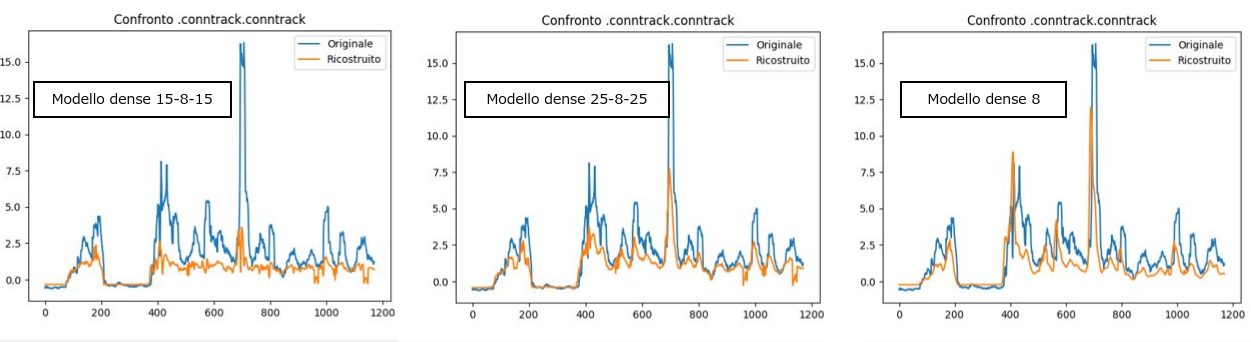
\includegraphics[width=\hsize]{images/my_work/confronto_modelli.png}
    \caption{Ricostruzione del grafico delle connessioni con diversi modelli.}
    \centering
\end{figure}

\paragraph{Reti LSTM} I risultati dei test relativi alle reti con nodi LSTM sono visibili nella tabella \ref{table:LSTM_tests}.


\begin{table}
    \begin{tabularx}{\textwidth}{||c X c c c c c c||} 
        \hline
        \# & Tipologia & 8-8-8-8 & 8-6-6-8 & 10-8-8-10 & 40-8-8-40 & 1& 1\\ [0.5ex] 
        \hline\hline
        1 & Syn Flood 100pps 40s & FN & FN & FN & FN & FN & FN \\ 
        \hline
        2 & Upload 500MB su Google Drive & TP & TP & TP & TP & TP & TP  \\ 
        \hline
        3 &  Download 600MB da Google Drive & TN  & TN & TN & TN & TN & TN \\ 
        \hline 
        4 & Normale mattinata & TN & TN & TN & TN & TN & TN \\
        \hline
        5 & Picco di traffico NTP & TN & TN & TN & TN & TN & TN \\
        \hline
        6 & Normale giornata & TN & TN & TN & TN & TN & TN \\ 
        \hline
        7 & Picchi di traffico NTP & TN & TN & TN & TN & TN & TN  \\ 
        \hline 
        8 & Syn Flood di 2min 50pps & TP & TP & TP & TP & TP & TP \\
        \hline
        9 & Syn Flood di 30s 50pps & FN & FN & FN & FN & TP & TP  \\        
        \hline
        10 & Port scanning (nmap) & TP & TP & FN & TP & TP & TP   \\
        \hline
        11 & ICMP Flood 100 pps & TP & TP & TP & TP & TP & TP \\
        \hline
        12 & UDP Flood 100pps & TP & TP & TP & TP & TP & TP \\ 
        \hline
        13 & DNS Amplification (4Mbps) & TP & TP & TP & TP & TP & TP \\ 
        \hline 
        14 & DNS Flood (4Mbps) & TP & TP & TP & TP & TP & TP \\
        \hline
        15 & Picco di connessioni (2500) & TN & TN & FP & FP & FP & FP\\        
        \hline 
        16 & Picco di connessioni & TN & TN & TN & TN & FP & TN\\        
        \hline
        17 & Picco di trasmissione & TN & TN & TN & TN & TN & TN\\        
        \hline
        18 & Connessioni alte & TN & TN & TN & TN & TN & TN\\
        \hline
        19 & Normale mattinata & TN & FP & TN & TN & FP & TN\\ 
        \hline
        20 & Pomeriggio con dei picchi di traffico NTP & TN & TN & TN & TN & TN & TN\\ 
        \hline
    \end{tabularx}
    \caption{Tabella dei risultati dei test con diversi modelli di reti neurali LSTM. TN=True Negative, TP=True Positive, FP=False Positive, FN=False Negative}
    \label{table:LSTM_tests}
\end{table}

I risultati sono buoni e paragonabili con i precedenti, ma una rete neurale ricorsiva richiede molto più tempo per essere allenata. Inoltre l'obiettivo principale di questa tesi non è la ricerca del modello di rete ottimale, quindi la scelta del modello è ricaduta su un modello denso, di quelli analizzati precedentemente. Per la messa in produzione del sistema verrà ricercato il modello ottimo.